%
% Chapter 7
%

\chapter{Signal Extraction and Systematic Uncertainties}
\label{sig_ext}
\epigraph{Statistics is the grammar of science.}{\textit{Karl Pearson}}
\vskip 0.5in
\section{Introduction}
The analysis is, in its essence, a sophisticated counting experiment. The presence of a signal is indicated by an excess of events over the predicted background, in the distribution of a signal variable. For our analyses the signal variables are collinear mass or BDT output, as described in chap~\ref{chap:event_sim} and~\ref{evt_sel}. Given that there are several uncertainties, both experimental and theoretical and also due to the innate randomness in the process, it is possible that an excess is observed when there is no signal. So, when an excess is observed, a p-value which represents the probability that the excess is due to statistical fluctuations is computed. A very low p-value is taken to indicate that the excess corresponds to an observed signal and not merely a statistical fluctuation. Conversely, if no excess is observed (upper exclusion) limits are set on the product of branching fraction and production cross-section. A 95\% CL (confidence level) is taken as a requirement for ruling out a signal at or above a certain value known i.e. upper exclusion limit. The first part of this chapter describes the statistical methods used, that very closely follow the procedure used for LHC Higgs boson search described in ~\cite{note2011}.

Several sources of systematic uncertainties need to be considered when making the above measurement. The sources of these uncertainties can be theoretical, experimental or purely statistical in nature. Further, they can affect only the overall scale of the distributions (used to make the measurement), or affect there shape i.e. change the scale differently in each bin of the distribution. All the uncertainties used in the analyses and their sources are described in the second part of this chapter.      



\section{Statistical methods for signal extraction}
\label{stat_meth}
In the following section, the expected signal event yields are denoted by $s$, and backgrounds by $b$. The parameter $\mu$ that appears below is the signal strength modifier, which changes the signal production cross-sections of all the production mechanisms by exactly the same scale $\mu$.

\subsection{Likelihood function}
The Poisson distribution is an appropriate model for n, the number of times an event occurs in an interval if the following assumptions are true~\cite{poisson_wiki}.
\begin{itemize}
\item The occurrence of one event does not affect the probability that a second event will occur. That is, events occur independently.
\item The rate at which events occur is constant. The rate cannot be higher in some intervals and lower in other intervals. This rate is the average number of events in the interval, $\lambda$.
\item Two events cannot occur at exactly the same instant; instead, at each very small sub-interval exactly one event either occurs or does not occur.
\end{itemize}
The poisson probability of distribution is then given by:
\begin{equation}
  P(n_{events})=\frac{e^{-\lambda}\lambda^{n}}{n!}
\end{equation}
For a counting experiments such as ours, the above conditions approximately hold. The expected number of events is $\mu\cdot s + b$. The likelihood function $\mathcal{L}(data|\mu)$ is then given by:
\begin{equation}
  \mathcal{L}(data|\mu)=\prod_{i=1}^{bins}\frac{(\mu\cdot s_i + b_i)^{n_i}}{n_{i}!}e^{-\mu\cdot s_i - b_i}
\end{equation}
where $n_i$ is the number of events observed in the bin i of the distribution, and $s_i$ and $b_i$ are expected number of signal and background events in that bin respectively.


\subsection{Treatment of systematic uncertainties}
\label{sys_treat}
All systematic uncertainties are handled by introducing them as nuisance parameters. Nuisance parameters are parameters that influence the model but are not of interest in our measurement, e.g., if we are interested in knowing only the mean of a population that is expected to be distributed as a gaussian, the standard deviation becomes a nuisance parameter for the model that we fit. In our experiment, the nuisance parameters are embedded into the likelihood function. In order for the likelihood function to have a clean factorized form~\cite{note2011}, all sources of uncertainties considered are taken to be 100\%-correlated or uncorrelated. If an uncertainty is partially correlated, it is either separated into 100\%-correlated or uncorrelated components, or considered 100\%-correlated or uncorrelated, depending on whichever is a more conservative estimate. The full suite of nuisance parameters is represented as $\theta$. These effect the expected signal and background yields which are now represented as $s(\theta)$ and $b(\theta)$. Each component of $\theta$ is associated with a default value $\tilde{\theta}$, reflecting our degree of belief on the real value of $\theta$. The pdf (probability distribution function) $\rho(\theta|\tilde{\theta})$ can then be interpreted as a posterior distribution from measurements of $\tilde{\theta}$. Using Bayes' theorem:
\begin{equation}
  \rho(\theta|\tilde{\theta})=\rho(\tilde{\theta}|\theta)\cdot\pi_\theta(\theta),
\end{equation}
where the priors $\pi_\theta(\theta)$ are taken as flat distributions representing no prior knowledge of $\theta$. This reformulation allows us to use the pdf of $\tilde{\theta}$ instead, i.e. $\rho(\tilde{\theta}|\theta)$  to directly constrain the likelihood of the measurement. The likelihood function after the introduction of systematic uncertainties now becomes:
\begin{equation}
  \mathcal{L}(data|\mu,\theta)=Poisson(data|\mu\cdot s(\theta) + b(\theta))\cdot\rho(\tilde{\theta}|\theta)
\end{equation}

Systematic uncertainties that effect only the overall scale of the distributions, correspond to a multiplicative factor in the signal and/or background yields, and are described by log-normal pdfs. Log-normal pdfs are characterized by the width $\kappa$, and are well-suited for positively valued observables. The log-normal distribution looks like:
\begin{equation}
\rho(\theta|\tilde{\theta})=\frac{1}{\sqrt{2\pi}\text{ ln}(\kappa)}\text{exp }(\frac{\text{ln}(\theta/\tilde{\theta})^2}{2(\text{ln }\kappa)^2}) \frac{1}{\theta}  
\end{equation}

Systematic uncertainties that effect the scale of the distribution differently in each bin have the effect of altering its shape along with its scale. Such uncertainties are called shape uncertainties ~\cite{shape_syst1}, and are modeled using a linear extrapolation method ~\cite{shape_syst2}. In practice, two alternate distributions obtained by varying the nuisance by $\pm 1$ standard deviation are used, and a parameter is added to the likelihood that smoothly interpolates between these shapes.

\subsection{Calculation of exclusion limits}
\label{exc_cal}
The CL$_\text{s}$ method~\cite{cls1,cls2,cls3} is used to set upper exclusion limits when no excess of data over background is observed. The test statistic used generally for hypothesis testing in searches at the LHC, uses profiling of nuisances as described above, and is based on the likelihood ratio~\cite{prof_likelihood}, which by the Neyman-Pearson lemma is known as the most powerful discriminator. This is denoted by $\tilde{q_\mu}$, and is given by:
\begin{equation}
\label{eq:proflik}
  \tilde{q_\mu}=-2\text{ ln}\frac{\mathcal{L}(\text{data}|\mu,\hat{\theta_\mu})}{\mathcal{L}(\text{data}|\hat{\mu},\hat{\theta})},\text{   with  } 0\leq \mu \leq \hat{\mu} 
\end{equation}
where $\hat{\theta_\mu}$ refers to the conditional maximum likelihood estimators of $\theta$, i.e. the set of nuisances parameters that maximize the likelihood for a given signal strength $\mu$, while $\hat\mu$ and $\hat\theta$ refer to the global maximum likelihood estimators for $\mu$ and $\theta$. The lower constraint on $\hat{\mu}$ i.e., $\hat{\mu}\geq 0$ ensures that the signal rate cannot be negative, while the upper constraint that $\hat{\mu}$, which is the global maximum value, cannot be less than the value of $\mu$ under consideration is imposed to guarantee that upward fluctuations of data such that $\hat{\mu}\geq \mu$ are not considered as evidence against the signal hypothesis, i.e., a signal of strength $\mu$.

Now, using equation~\ref{eq:proflik}, the observed value of the test statistic, $\tilde{q_\mu}^{obs}$, is calculated for the signal strength $\mu$. Also, maximum likelihood estimators for the nuisance parameters, for the background-only($\mu=0$) and signal-plus-background(current $\mu>0$ under consideration) hypotheses are calculated. They are denoted by $\hat{\theta_{0}}^{obs}$ and $\hat{\theta_\mu}^{obs}$ respectively, and are used to generate toy Monte Carlo pseudo-datasets. These pseudo datasets are used to construct  pdfs, using equation~\ref{eq:proflik}, of test statistics $f(\tilde{q_\mu}|0,\hat{\theta_{0}}^{obs})$ and $f(\tilde{q_\mu}|\mu,\hat{\theta_\mu}^{obs})$ by treating them as they were real data. Example of these distributions are shown in Fig.~\ref{fig:test_stat_dist}.
\begin{figure*}[!htpb]\centering
 \captionsetup{width=.87\textwidth,justification=centering}
 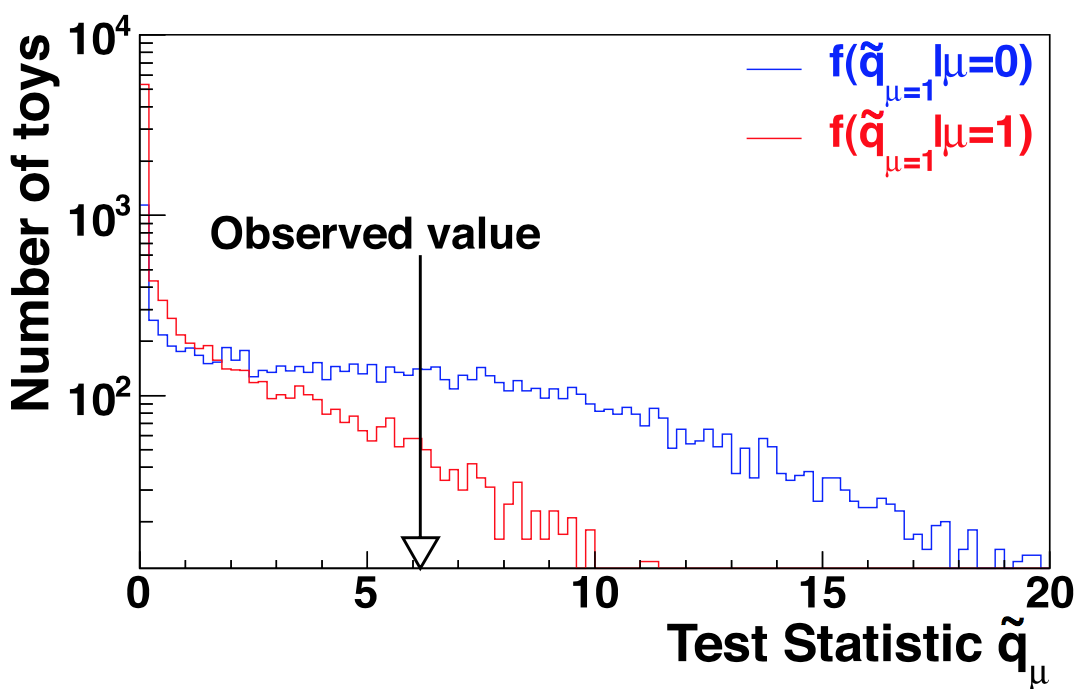
\includegraphics[width=0.85\textwidth]{plots_and_figures/chapter7/test_statistic_distri.png}
 \caption{Test statistic distributions for ensembles of pseudo-data generated for signal-plus-background (red) and background-only (blue) hypotheses~\cite{note2011}.}
 \label{fig:test_stat_dist}
\end{figure*}


Having constructed the above pdfs, it is now possible to calculate the probabilities of the observations under both hypotheses. The first quantity that we calculate is:
\begin{equation}                                                                                                                                                                                                 \label{eq:pmu}                                                       p_\mu=P(\tilde{q_\mu}\geq \tilde{q_\mu}^{obs}|\text{signal-plus-background})=\int_{\tilde{q_\mu}^{obs}}^{\inf}f(\tilde{q_\mu}|\mu,\hat{\theta_\mu}^{obs})d\tilde{q_\mu}
\end{equation}

The above quantity corresponds to CL$_\text{s+b}$ and measures the incompatibility of data with signal-plus-background hypothesis. This quantity alone is not adequate for hypothesis testing in situations when the signal is so small that both hypotheses are compatible with the observation and a downward fluctuation of the background can lead to an inference of signal.

The second quantity we calculate is:
\begin{equation}                                                                                                                          
  \label{eq:pb}                                                     
  1-p_b=P(\tilde{q_\mu}\geq \tilde{q_\mu}^{obs}|\text{background-only})=\int_{\tilde{q_\mu}^{obs}}^{\inf}f(\tilde{q_\mu}|0,\hat{\theta_0}^{obs})d\tilde{q_\mu}                                                                                                            
\end{equation}
This quantity corresponds to CL$_\text{b}$ and measures the incompatibility of data with the background. The incompatibility of the data with background-only hypothesis alone doesn't tell us that it is indeed compatible with the signal, and so is not considered a good test of the signal hypothesis.

The ratio of the two quantities referred to as CL$_\text{s}$~\cite{cls1,cls2,cls3} helps deal with both situations above well, and is given by:
\begin{equation}                                                                                                                          
  \label{eq:cls}                                                                                                                           \text{CL}_\text{s}=\frac{p_\mu}{1-p_b}
\end{equation}

The 95\% CL is then arrived at by iterating over $\mu$ until we have CL$_\text{s}=0.05$. And the amount of signal or above, given by that $\mu$, denoted as $\mu^{95\%CL}$, is said to be excluded at 95\% CL. 

\subsection{Median expected limits}

Upper exclusion limits calculated using toy datasets of background-only expectation, are called expected limits. A large set of background-only pseudo-data is generated, and CL$_\text{s}$ and $\mu^{95\%CL}$ is calculated for each of them. The median expected limit is calculated by integrating over this distribution until the 50\% quantile is reached. The $\pm 1\sigma$ and $\pm 2\sigma$ bands are calculated similarly by integrating the distribution to the appropriate quantiles are reached. The calculation of median expected limits does not involve using the observed data and hence can be calculated when the analyses is blinded to prevent experimenter's bias (as mentioned in Section~\ref{evt_sel_intro}). This can be use to maximize the sensitivity of the search, as described in Sections~\ref{h125_cb_sel} and ~\ref{H125_cb_sel}. A more stringent (lower) median limit corresponds to a more sensitive search.  


\subsection{Quantifying an excess of events}
\label{theo_uncert}
In case an excess of data over background is observed, it is necessary to make sure beyond a reasonable doubt that the excess is not merely a fluctuation. This is quantified using the background-only p-value, which is the probability for the background to fluctuate and give an excess of events as large or larger than that observed. The same test statistic as equation~\ref{eq:proflik} is used with the signal strength set to 0 to correspond to the background-only hypothesis:

\begin{equation}
\label{eq:proflik_b}
  \tilde{q_0}=-2\text{ ln}\frac{\mathcal{L}(\text{data}|0,\hat{\theta_0})}{\mathcal{L}(\text{data}|\hat{\mu},\hat{\theta})},\text{   with  } 0\leq\hat{\mu} 
\end{equation}
The constraint on $\hat\mu$ being greater than 0 is required so that a deficit of events in observed data is not interpreted in the same manner as we would an excess. In other words a departure from the background hypothesis in the form of deficit of events is not considered in favor of the signal hypothesis. Following the same procedure as calculation of observed limits (as described in~\ref{exc_cal}) and generating pseudo-data, the distribution $f(\tilde{q_0}|0,\hat{\theta_{0}}^{obs})$ is constructed. The p-value is then given by:

\begin{equation}                                                                                                                          
  \label{eq:p0}                                                     
  p_0=P(\tilde{q_0}\geq \tilde{q_0}^{obs})=\int_{\tilde{q_0}^{obs}}^{\inf}f(\tilde{q_0}|0,\hat{\theta_0}^{obs})d\tilde{q_0}               \end{equation}

The p-value can be converted to significance $\mathcal{Z}_0$, which is an equivalent way of quantifying an excess and is related to the p-value by the following:

\begin{equation}                                                                                                                          
  \label{eq:sig}                                                                                                                           p_0=\int_{\mathcal{Z}_0}^{\inf}\frac{1}{\sqrt{2\pi}}exp(-x^2/2)dx
\end{equation}

Broadly, the significance corresponds to how far into the tail of the distribution (i.e., away from the most probable value), assuming background hypothesis, the test statistic value corresponding to the observed data lies. The farther it is, the less likely it is to have been a fluctuation. The conventional standard in high energy physics to be able to claim observation of a process is a significance of $5\sigma$, which corresponds to a p-value of $2.8\times 10^{-7}$.


\section{Systematic uncertainties}
\label{exp_uncert}
It is important to consider all relevant sources of uncertainties when performing sophisticated counting experiments such as these. Uncertainties that are introduced as a result of imprecise/inaccurate knowledge of the system or gaps in prior knowledge that is used in the measurement are called systematic uncertainties. They are a different class of uncertainties than those arising purely out randomness in statistical measurements, called statistical uncertainties. The sources of systematic uncertainties range from purely theoretical in nature to purely experimental. They can be categorized in the two following ways:
\subsection{Normalization uncertainties}
The value of these uncertainties are independent of the signal/discriminant variable. To be more precise, these uncertainties are independent of the value of $\mcol$ or BDT response. Hence, they effect each bin of those distributions in exactly the same manner and thus change only the overall scale of the distribution without altering its shape.

The muons in the analysis are required to pass certain identification, isolation and triggering criteria (see chapter~\ref{evt_sel}). The efficiencies for muon to pass these criteria are measured via tag-and-probe methods~\cite{muon_recon2018} using $Z\rightarrow\Pgm\Pgm$ events, and the scale factors are used to match the efficiency in MC to that in data (see section~\ref{anal_trigger}). The efficiencies determined by this process, like any other quantity, are associated with systematic  uncertainties. For the muons used in the analyses described here, a combined normalization uncertainty of 2\% is associated with muon trigger, identification and isolation. Similar to muons, the efficiencies for electrons used in the analyses have also been measured via tag-and-probe methods~\cite{e_recon} using $Z\rightarrow\Pe\Pe$ events. The uncertainties in efficiencies  of electron identification and isolation criterion are also included as a normalization uncertainty of 2\% in the fit. Both the above uncertainties are applied to processes which are derived from MC simulation. As mentioned earlier, a b tagging veto is applied in the analysis in order suppress backgrounds involving top quarks. The efficiency of b tagging procedure is different in MC simulation than data. A scaling procedure is applied to match these efficiencies, and the uncertainties associated with these factors are found to not effect the shape of the $\mcol$ or BDT distributions. They are thus included in the fit as normalization uncertainties and range across categories from 2-4.5\% and 2-2.5\% for $\hmue$ and $\Hmue$ analysis respectively.

Several backgrounds in the analyses are estimated using MC simulations (see chapter ~\ref{bg_val}). These include \ztt, \ttb, \wjets, $\PW\PW$, $\PW\PZ$ and $\PZ\PZ$, $Z\to\ell\ell$ $(\ell = \Pe, \Pgm)+\text{jets}$, single-top quark production, $\PW\gamma^{(*)}+\text{jets}$. The production cross-sections for these backgrounds determine the number of events each background would contribute. These cross-sections are measured experimentally and the uncertainty in those measurements are included in the fit. Given that a change in cross-section changes the overall number of events produced, it has no effect on the shape of distributions. Hence these uncertainties are included as normalization uncertainties. These uncertainties in general  arise from: uncertainties on the parton distribution functions and strong coupling constant (called PDF+$\alpha_s$); variations in renormalization and factorization scales. In the $\Hmue$ analysis a separate uncertainty is applied for PDF+$\alpha_s$ and renormalization/factorization scales for each of the backgrounds. In $\hmue$ analysis, a combined uncertainty for each background is applied to cover both sources. All the above uncertainties are considered 100\% correlated among categories. For each background, a 5\% uncertainty, uncorrelated among all categories, is also applied to conservatively cover differences across categories. The QCD multijet background is estimated using a data-driven procedure. An uncertainty of 30\% associated with this procedure (corresponding to the uncertainty in the extrapolation factor from the same-sign to opposite-sign region) is included in the fit. All uncertainties are summarized in table ~\ref{table:syst}~\cite{HIG-17-001,HIG-18-017}. All uncertainties in the table are treated as correlated between the categories, except those with more values separated by the $\oplus$~symbol. In the case of two values, the first value is the correlated uncertainty and the second value is the uncorrelated uncertainty for each individual category. In the case of three values, the  first and second values correspond to the uncertainties arising from factorization and renormalization scales and PDF variations and are correlated between categories, while the third value is the uncorrelated uncertainty for each individual category. Two values separated by the ``--'' sign represent the range of the uncertainties from the different sources and/or in the different jet categories.

\begin{table}[htpb]
  \begin{center}
    \caption{The systematic uncertainties for both analyses
      (see text for explanation of the $\oplus$~symbol)}
\begin{tabular}{l*{2}{c}} \hline
Systematic  uncertainty            & $\hmue$& $\Hmue$  \\ \hline
Muon  trigger/ID/isolation         &          2\%           &        2\%         \\
Electron trigger/ID/isolation      &          2\%           &        2\%           \\
b tagging veto                     &      2.0--4.5\%        &      2.0--2.5\%         \\ 
[\cmsTabSkip]
QCD multijet background            &          30\%          &        30\%                \\
$\ztt+\textrm{jets}$ background    &    10\%$\oplus$5\%     & 0.1\%$\oplus$2\%$\oplus$5\%         \\
$\ttb$ background                  &    10\%$\oplus$5\%     &   10\%$\oplus$5\%              \\
$W+\textrm{jets}$ background       &    10\%$\oplus$5\%     & 0.8\%$\oplus$3.8\%$\oplus$5\%        \\
$\PW\PW,\PZ\PZ,\PW\PZ$ background  &    5\%$\oplus$5\%      &  3.5\%$\oplus$5\%$\oplus$5\%       \\
$\PW\gamma^{(*)}$ background       &    10\%$\oplus$5\%     &  10\%$\oplus$5\%       \\
Single top quark background        &    5\%$\oplus$5\%      & 3\%$\oplus$5\%$\oplus$5\%    \\ 
$Z\to\Pgm\Pgm/\Pe\Pe$ background   &    10\%$\oplus$5\%     & 0.1\%$\oplus$2\%$\oplus$5\%     \\
[\cmsTabSkip]
Jet energy scale                   &        3--20\%         &        3--20\%                         \\
$\Pgm$ energy scale                &        0.2\%           &        0.2\%                              \\
 $\Pe$ energy scale                &        0.1--0.5\%      &        0.1--0.5\%                          \\
Unclustered energy scale           &        $\pm 1 \sigma$  &     $\pm 1 \sigma$                            \\
pileup                             &        $\pm 1 \sigma$  &     $\pm 1 \sigma$                            \\
[\cmsTabSkip]
Integrated luminosity              &         2.5\%          &       2.5\%                                        \\ \hline
\end{tabular}
\label{table:syst}
\end{center}
\end{table}


Just like MC backgrounds described above, the signal in both $\hmue$ and $\Hmue$ analysis comes from MC simulation. The signal process and the SM Higgs background are associated with uncertainties in the Higgs boson production cross sections. These come from variations in factorization/renormalization scales, as well as PDF+$\alpha_s$, and result in changes only in normalization. These uncertainties are summarized for SM Higgs boson and heavier Higgs of different masses in table~\ref{table:syst}. They are taken from Handbook of LHC Higgs cross-sections found in Ref.~\cite{YR4}. The PDF and $\alpha_s$ uncertainties are computed following the recommendation of the PDF4LHC working group. The remaining Gaussian uncertainty accounts for additional intrinsic sources of theory uncertainty described in detail in the reference~\cite{HIG-18-017}.

\begin{table}[!htbp]
  \begin{center}
  \caption{ Theoretical uncertainties applied to the Higgs boson production cross sections for the different masses}
  \begin{tabular} {cccc}
    \hline
    $m_{\PH}$  (GeV) &Production mode&Theory, Gaussian (\%) & PDF$+\alpha_s$  (\%)\\\hline
125 & GGF&$\pm$3.9
&$\pm$3.2\\
125 & VBF&$\pm$0.4
&$\pm$2.1\\
200 & GGF &$\pm$1.8
&$\pm$3.0\\
300&GGF&$\pm$1.8
&$\pm$3.0\\
450&GGF
&$\pm$2.0
&$\pm$3.1\\
600&GGF
&$\pm$2.1
&$\pm$3.5\\
750&GGF
&$\pm$2.1
&$\pm$4.0\\
900&GGF
&$\pm$2.2
&$\pm$4.6\\\hline
  \end{tabular}
  \label{tabe:syst_signal}
\end{center}
\end{table}



The estimation of a particular background, that is derived from simulation, needs to correspond to the number of events (of that background, having a particular cross-section) that would be produced in the amount of proton-proton collision data that we are using for this search. In other words, the background estimations need to be normalized to (brought to the same scale as) the integrated luminosity of the data collected. This integrated luminosity (defined in chapter~\ref{chap:exper_setup}) is a measured quantity, and like all measured quantities, has an uncertainty associated with it. This amounts to 2.5\% and, like other normalization uncertainties, only effects only the overall scale of distributions.  




\subsection{Shape uncertainties}
In this section, we describe the systematic uncertainties which not only alter the scale but also the shape of the distributions. We start with the description of uncertainties associated with jet energy corrections. As described in Section~\ref{jet_recon}, the reconstruction of complex objects such as jets need to corrected using several correction factors. These factors have uncertainties associated with them and these are included in the fit as shape uncertainties. There are several different sources of these uncertainties and the effect of each is propagated to the fit by including alternate distributions for each process where each source of uncertainty has been moved by one standard deviation on either side. The effect of changing these sources is propagated through the jets in the analysis, and also other affected quantities such as the \ptmiss. A total of 27 sources are considered, and these include effects of pileup, composition of jets, $\eta$ dependence etc. They vary in the range from 3-20\% and are considered uncorrelated.

Just like jets, there are shape uncertainties associated with the energy scale of electrons and muons. The effect of electron energy scale uncertainty is treated in a similar manner by propagating the effect of varying the scale to process distributions which are then included in the fit. The uncertainties are a result of the sum in quadrature of the following components: electron selection efficiency, pseudorapidity dependence, and shower-shape related categorization. The resolution systematics result to be negligible and are thus not considered in the fit. The value of this uncertainty ranges from 0.1-0.5\%. The muon energy scale uncertainty amounts to 0.2\% and is treated in the same manner as above.

Jets with $\pt<15$ GeV or PF candidates which do not get clustered inside any jets are called unclustered energy. Their scale that effects the \ptmiss in particular, and is associated with a shape uncertainty that is treated the same way as others~\cite{Sirunyan:2019kia}. Four sources of unclustered energy scale uncertainty are considered, and estimated independently for these four particle categories: charged particles, photons, neutral hadrons, and HF (very forward, high $|\eta|$) particles which are not contained in jets. The effect of these sources on the unclustered energy is propagated in the same manner as described above, and they are considered uncorrelated.

A set of weights is applied in order make the distribution of pileup in MC simulation match that of pp collision data. There is an uncertainty associated with this process. This is included  by varying the weights by changing by 5\%, in each direction, the total inelastic cross section used in the estimation of the pileup events in data~\cite{Sirunyan:2018nqx}. These new set of weights are then applied event-by-event, producing alternate distributions that are included in the fit as shape uncertainties.

A shape uncertainty is also considered to deal with the fact that purely statistical fluctuations can change the shape of the distribution. These uncertainties are called bin-by-bin uncertainties as they account for statistical uncertainty in every bin of the distribution. Alternate distributions are created by varying the contents of each bin up and down, and these distributions are included in the fit as shape uncertainties~\cite{BARLOW}. Given that considering all bins of all processes will result in a very large number of such nuisances being considered, shape uncertainties for only those bins are considered in which there is more than 10\% variation in the up and down shift. All shape uncertainties are summarized in Table~\ref{table:syst}.


% % uncomment the following lines,
% if using chapter-wise bibliography
%
% \bibliographystyle{ndnatbib}
% \bibliography{example}


